\setAuthor{Mihkel Kree}
\setRound{lõppvoor}
\setYear{2009}
\setNumber{G 1}
\setDifficulty{2}
\setTopic{Staatika}

\prob{Nürinenud käärid}
Juku asus hekikääridega õunapuult jämedat kuivanud oksa lõikama. Et aga käärid olid juba ammu nürinenud, polnud neist mingit abi. Enamgi veel, oks hakkas kääride kokkuvajutamise ajal terade vahel lausa libisema. Libisemine peatus hetkel, mil terade vaheline nurk oli kahanenud $\alpha$-ni. Kui suur oli hõõrdetegur oksa ja nürinenud lõiketera vahel?

\hint
Toereaktsiooni kääride telje sihiline komponent peab olema tasakaalustatud hõõrdejõu poolt.

\solu
\begin{center}
	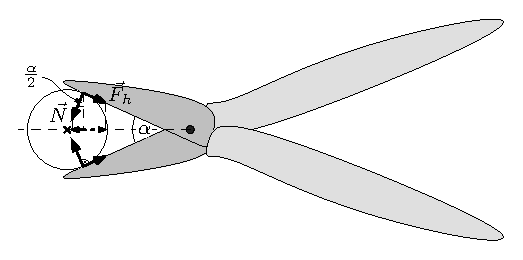
\includegraphics[width=0.9\linewidth]{2009-v3g-01-G_nyrinenud_kaarid_lah.eps}
\end{center}

Hõõrdejõud peab tasakaalustama toereaktsiooni kääride telje sihilise komponendi (joonis). Lihtsast geomeetriast saame, et $\mu = \tan \frac{\alpha}{2}$.
\probend